\documentclass[
twocolumn,
% hf,
]{ceurart}

%%
%% One can fix some overfulls
\sloppy

%%
%% Minted listings support 
%% Need pygment <http://pygments.org/> <http://pypi.python.org/pypi/Pygments>
\usepackage{minted}
%% auto break lines
\setminted{breaklines=true}

%% strikethrough
\usepackage[normalem]{ulem}

\usepackage{tikz}
\usepackage{graphicx}

\usepackage{listings}
\lstset{columns=flexible,tabsize=2}

\newcommand*{\class}[1]{\textsc{#1}}
\newcommand*{\feature}[1]{\emph{#1}}
\newcommand*{\file}[1]{\texttt{#1}}

%ATL language highlighting
\lstdefinelanguage{atl}
  {morekeywords={module, create, from, to, using, mapsTo, rule, helper, refining, lazy,
                 context, def, if, then, else, endif, library, and, or, not, query, do,
                 unique, extends},
   sensitive=false,
   morecomment=[l]{--}}

%Standard listing style
\lstset{basicstyle=\ttfamily\small,keywordstyle=\sffamily\small\textbf}

\begin{document}

%%
%% Rights management information.
%% CC-BY is default license.
\copyrightyear{2023}
\copyrightclause{Copyright for this paper by its authors.
  Use permitted under Creative Commons License Attribution 4.0
  International (CC BY 4.0).}

%%
%% This command is for the conference information
\conference{TTC'23: 15th Transformation Tool Contest, 
  Part of the Software Technologies: Applications and Foundations (STAF) federated conferences,
  Eds. A. Boronat, A. Garc\'{i}a-Dom\'{i}nguez, and G. Hinkel,
  20 July 2023, Leicester, UK.}

\title{The TTC 2023 KMEHR to FHIR case}
\author[1]{Dennis Wagelaar}[%
email=dennis.wagelaar@corilus.be
]
\address[1]{  Corilus nv,
  Gaston Crommenlaan 4, 9050 Gent}

\maketitle

\begin{abstract}
The history of medical information systems has seen many twists and turns, and 
while there has long been a global standardization body in the form of HL7, it 
only recently gained a lot of traction with the FHIR standard. As a result, a 
number of countries have developed their own medical data interchange formats 
over the years, which now need to be realigned with the global FHIR medical 
data interchange format. One such example is the Belgian KMEHR format. 
For this TTC case, we will focus on a specific kind of medical data 
interchange, namely the Patient Summarized Medical Record. In KMEHR, this is 
called the Summarized Electronic Health Record (SumEHR). In FHIR, this is 
called the International Patient Summary (IPS). The primary purpose of such a 
record is to provide an emergency ``cheat sheet'' to healthcare providers who 
don't normally see the patient in question, e.g. a hospital's emergency 
department. Especially when a patient is abroad, the capability to exchange 
such data is important, as it will often be the only source of medical 
background data. This TTC case will require you to translate between the 
Belgian SumEHR format and the international FHIR IPS format.
\end{abstract}

\section{Introduction}

This Transformation Tool Contest case concerns the transformation between two
medical data interchange formats: the Belgian ``Kindly Marked-up Electonic
Healthcare Record'' (KMEHR) standard~\cite{kmehr_2023}, and the international
``Fast Healthcare Interoperability Resources'' (FHIR) standard by Health Level
7 (HL7)~\cite{fhir_2023}.

For this TTC case, we will focus on a specific kind of medical data 
interchange, namely the Patient Summarized Medical Record. In KMEHR, this is 
called the Summarized Electronic Health Record (SumEHR)~\cite{sumehr_2016}.
In FHIR, this is called the International Patient Summary
(IPS)~\cite{fhirips_2022}. The primary purpose of a Patient Summarized Medical
Record is to provide an emergency reference sheet to healthcare providers who 
don't normally see the patient in question, e.g. a hospital's emergency 
department, or a different doctor than your regular doctor.
Especially when a patient is abroad, the capability to exchange 
such data is important, as it will often be the only source of medical 
background data.

All resources for this case are available on
Github\footnote{\url{https://github.com/dwagelaar/ttc2023-kmehr2fhir}}.
Please follow the link in the footnote and create a pull request with your own
solution.

The rest of the document is structured as follows:
Section~\ref{sec:case-structure} describes the structure of the KMEHR to FHIR 
case. Section~\ref{sec:task-description} describes the proposed tasks for this
case. Section~\ref{sec:benchmark-framework} mentions the benchmark framework for
those solutions that focus on raw performance. Finally,
Section~\ref{sec:evaluation} mentions an outline of the initial audience-based
evaluation across all solutions, and the approach that will be followed to
derive additional prizes depending on the attributes targeted by the solutions.

\section{Case Structure}
\label{sec:case-structure}

The case is intended to review the different approaches for bridging the gap
between two medical data standards, KMEHR and FHIR, that use vastly different
document structures and medical code systems. The metamodels for
KMEHR and FHIR have been automatically generated from their published XML 
schemas\footnote{FHIR canonically uses JSON
representation, but the standard also provides an XML representation.}
using the EMF XSD generator\footnote{\url{https://help.eclipse.org/latest/index.jsp?topic=\%2Forg.eclipse.emf.doc\%2Ftutorials\%2Fxlibmod\%2Fxlibmod.html}}.
The resulting metamodels are too large to include in this paper, but they
can be viewed online at the
``kmehr-emf''\footnote{\url{https://github.com/dwagelaar/kmehr-emf}} and
``fhir-xml-emf''\footnote{\url{https://github.com/dwagelaar/fhir-xml-emf}}
Github projects. The metamodels consist of 297 and 1110 metaclasses,
respectively. Please note that the original XSD files are also included
in these GitHub repositories.

These metamodels aren't only large because they cover many concepts, but also
due to accidental complexity that is caused mostly by the process of a large
standardization body, and to a lesser extent by EMF's representation in Ecore
of XML schemas. It is necessary for an industrial transformation tool to be
able to process the technical space~\cite{conf/gttse/Bezivin2005} that is
used, and not require the end user to manually translate from the provided
technical format to the modeling technology of choice.
Having to bridge technical spaces is common for industrial data format standards,
which often don't target modeling technology. It is also apparent that the
level of accidental complexity is proportial to the size of the standardization
body, as can be seen in the size difference between the KMEHR and FHIR
metamodels. FHIR simply has a much larger scope, and must be general enough
to apply worldwide. It therefore also covers many more corner cases than
KMEHR.

Figure~\ref{fig:fhirextract} shows
a small part of the FHIR metamodel that shows how primitive types, such as
strings, integers, and booleans, are wrapped inside a container object.
The KMEHR metamodel does not do this, and an additional translation step
is necessary to bridge this -- purely technical -- gap. In this case,
the Composition metaclass, which represents the body of the medical record
summary, typically has a custodian. The custodian is the medical party that
is responsible for keeping the medical record summary up to date, and is
typically your general practitioner in Belgium. The custodian property is
represented as a reference string in FHIR, which resolves to the type and
identifier of a Resource (document attachment) inside the same FHIR
Bundle (document).

\begin{figure}[ht]
\centerline{
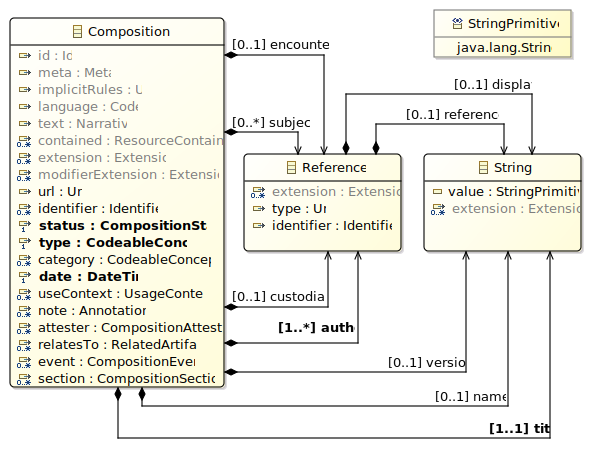
\includegraphics[width=7.5cm]{figures/fhirextract}}
\caption{Extract of the FHIR metamodel}
\label{fig:fhirextract}
\end{figure}

A transformation tool's ability to deal with this accidental complexity is an
important factor for industrial acceptance. Not only should the transformation
tool be able to process the accidental complexity, but it should also allow
the user to hide away or otherwise modularize the part of the transformation
code/specification that deals with this accidental complexity.

The reference transformation is written in ATL/EMFTVM~\cite{conf/models/Wagelaar2011}
and comprises approximately 1300 lines of code, divided over the main \texttt{KMEHRtoFHIR.atl}
transformation module and the \texttt{libKMEHRtoFHIR.atl} helper library. Both
of these files can be found in the aforementioned case Github repository. It uses
advanced features of the EMFTVM runtime, such as multiple rule inheritance and
invocation of native Java code. It also relies on the local search compiler
included with the 4.8.0 release of ATL, which allows for efficient
execution of matched rules with many input element. For example, the Posology
rule shown in Listing~\ref{lst:posologyRule} uses four input elements, which would
require iterating four times through the entire input model before ATL 4.8.0.
As of ATL 4.8.0, the filter expressions on lines 7--9 are translated by the compiler
into local search expressions for the \texttt{tx}, \texttt{i}, and \texttt{s} input
elements. Only the \texttt{f} input element needs to be found by iterating over
the entire input model. An additional \textbf{mapsTo} keyword is required to
indicate that the output element \texttt{t} does not map to the entire collection
of input elements, as is the default, but rather directly maps to the input
element \texttt{s}. That way, whenever another transformed model element is
assigned a reference to KMEHR!PosologyType \texttt{s}, ATL's implicit tracing
mechanism will translate it to FHIR!MedicationStatement \texttt{t}.

\begin{lstlisting}[
  float,frame=tb,
  breaklines,language=atl,mathescape,
  caption=Posology rule,label={lst:posologyRule}
]
rule Posology {
	from
		f : KMEHR!FolderType,
		tx : KMEHR!TransactionType,
		i : KMEHR!ItemType,
		s : KMEHR!PosologyType (
			i.posology = s and
			tx.item->includes(i) and
			f.transaction->includes(tx) and
			i.isMedication)
	to
		t : FHIR!MedicationStatement mapsTo s (
			id <- msid,
			medication <- medCodRef,
			status <- msstatus,
			subject <- subRef,
			effectivePeriod <- effectivePeriod,
			dosage <- Sequence{dosage}),
		msid : FHIR!Id (
			value <- s.uuid),
		medCodRef : FHIR!CodeableReference (
			reference <- medRef),
		medRef : FHIR!Reference (
			reference <- thisModule.FhirString('Medication/' + i.uuid)),
		msstatus : FHIR!MedicationStatementStatusCodes (
			value <- #recorded),
		subRef : FHIR!Reference (
			reference <- thisModule.FhirString('Patient/' + f.patient.uuid)),
		effectivePeriod : FHIR!Period (
			start <- thisModule.FhirDateTime(i.beginmoment),
			end <- thisModule.FhirDateTime(i.endmoment)),
		dosage : FHIR!Dosage (
			timing <- timing),
		timing : FHIR!Timing (
			repeat <- repeat),
		repeat : FHIR!TimingRepeat (
			count <- thisModule.FhirPositiveInt(i.dayperiod->size()),
			periodUnit <- periodUnit,
			when <- i.dayperiod->collect(dp | thisModule.EventTiming(dp))),
		periodUnit : FHIR!UnitsOfTime (
			value <- #d)
}
\end{lstlisting}

The Posology rule is responsible for translating the statement of how and when
medication must be administered -- e.g. ''once daily, after dinner''
-- from a KMEHR!PosologyType to a FHIR!MedicationStatement, as well as during
which time period it is applicable (the \texttt{effectivePeriod}). Another
transformation rule PosologyWithUnitAndTakes exists, which extends the Posology
rule by adding a unit and dosage, e.g. ''1 caps.''. This rule is shown in
Listing~\ref{lst:posologyWithUnitAndTakesRule}.

\begin{lstlisting}[
  float,frame=tb,
  breaklines,language=atl,mathescape,
  caption=Posology rule,label={lst:posologyWithUnitAndTakesRule}
]
rule PosologyWithUnitAndTakes extends Posology {
	from
		f : KMEHR!FolderType,
		tx : KMEHR!TransactionType,
		i : KMEHR!ItemType,
		s : KMEHR!PosologyType (
			not s.unit.oclIsUndefined() and
			not s.takes.oclIsUndefined()
		)
	to
		t : FHIR!MedicationStatement mapsTo s,
		doseAndRate : FHIR!DosageDoseAndRate (
			type <- thisModule.CodeableConcept(thisModule.CodingWithDisplay(
				'http://terminology.hl7.org/CodeSystem/dose-rate-type',
				'ordered',
				'Ordered'
			)),
			doseQuantity <- doseQuantity
		),
		dosage : FHIR!Dosage (
			doseAndRate <- Sequence{doseAndRate}
		),
		doseQuantity : FHIR!Quantity (
			system <- qSys,
			code <- qCode,
			unit <- thisModule.FhirString(s.unit.cd.toUnitsOfMeasureValue),
			value <- thisModule.FhirDecimal(s.takes.high)
		),
		qSys : FHIR!Uri (
			value <- 'http://unitsofmeasure.org'
		),
		qCode : FHIR!Code (
			value <- '1'
		)
}
\end{lstlisting}

Note how ATL modularizes the accidental complexity of wrapped primitive types
in FHIR by delegating the creation of the wrapper objects to lazy rules, such
as the FhirString rule shown in Listing~\ref{lst:fhirStringRule}. The Posology rule
can now simply wrap the medication reference string inside a FHIR String by
invoking the lazy rule. Note that the remaining medication reference wrapper
objects, CodeableReference and Reference, could also have been modularized
in a lazy rule, further increasing the clarity of the Posology rule. This
has not been done here, because those wrapper objects are only used once
in the entire transformation code. Instead, only the wrapper objects that
must be created several times are extracted into lazy rules.

\begin{lstlisting}[
  float,frame=tb,
  breaklines,language=atl,mathescape,
  caption=Posology rule,label={lst:fhirStringRule}
]
lazy rule FhirString {
	from
		s : String
	to
		t : FHIR!"fhir::String" (
			value <- s
		)
}
\end{lstlisting}

The transformation translates a SumEHR document, which is effectively a KMEHR
document with a header and a folder that contains administrative patient
data and a ``sumehr'' type transaction. The sumehr transaction contains a
number of items of the following types:

\begin{itemize}
\item \textbf{gmdmanager}: the doctor that is responsible for keeping the
  patient's main medical record up-to-date. It is translated to a custodian
  Practitioner element in FHIR.
\item \textbf{contactperson}: a key contact person of the patient, such
  as a family member or employer. It is translated to a list of contact
  CodeableConcepts in FHIR, embedded within the Patient element.
\item \textbf{socialrisk}: a health-related risk originating from the
  patient's social context. It is not included in a FHIR IPS document.
\item \textbf{risk}: a health-related general risk for the patient.
   It is not included in a FHIR IPS document.
\item \textbf{problem}: an ongoing condition the patient suffers from,
  or -- if inactive -- a historic condition. It is translated to a
  Condition element in FHIR.
\item \textbf{medication}: currently prescribed medication for the patient.
  It is translated to a Medication element in FHIR, with the embedded
  KMEHR Posology being translated to a MedicationStatement element in
  FHIR.
\item \textbf{vaccine}: a vaccine/immunization the patient has received
  in the past. It is translated to an Immunization element in FHIR.
\item \textbf{adr}: an adverse drug reaction that the patient suffers from.
  It is translated to an AllergyIntolerance element of type ''intolerance''
  in FHIR.
\item \textbf{allergy}: an allergy the patient suffers from.
  It is translated to an AllergyIntolerance element of type ''allergy''
  in FHIR.
\end{itemize}

More types of information could be included in both SumEHR and FHIR IPS, but
for the purpose of the TTC case, the types are limited to the ones listed.

In addition, the reference model transformation does not (fully) translate
between the medical coding systems used in KMEHR and FHIR for the sake of
simplicity, and simply embeds the KMEHR medical codes within the FHIR document.
Submissions to this case should follow the same strategy.

That said, a full translation would have to map additional medical
coding systems in order to be complete, notably units of
measure\footnote{\url{http://unitsofmeasure.org}} and vaccine indication
codes\footnote{\url{https://www.ehealth.fgov.be/standards/fhir/vaccination/ValueSet-be-vs-vaccine-code.html}}.
Finally, a translation of the Belgian CNK codes for medication to the
international ATC standard would be very useful, but that would require
incorporating a database in the transformation, such as SAM\footnote{\url{https://www.samportal.be/}}.

\section{Task Description}
\label{sec:task-description}

There is a mandatory task and an optional task in this case:

\begin{itemize}
\item The mandatory task is to re-implement or improve the original
  transformation itself, in a way that lends itself better to after-the-fact
  consistency checking. Your transformation tool may have better support for
  this, or ATL could be made to deal better with larger versions of this model.

\item The optional task is to define the reverse transformation that translates
  the generated FHIR IPS document back to SumEHR.
\end{itemize}

Solutions can focus on efficiency, conciseness, or clarity of presentation to
the user. Clarity of presentation is key for this kind of transformation, as
domain experts must typically validate the correctness of the transformation
logic by reviewing the code.

\section{Benchmark Framework}
\label{sec:benchmark-framework}

If focusing on performance, the solution authors should integrate their solution
with the provided benchmark framework. It is based on that of the TTC 2017 Smart
Grid case~\cite{hinkel_ttc_2017}, and supports the automated build and execution
of solutions. For this specific case study, the visualisation of the results is
currently disabled.

The benchmark consists of three phases:

\begin{enumerate}
\item \textbf{Initialization}, which involves setting up the basic
  infrastructure (e.g. loading metamodels). These measurements are optional.
\item \textbf{Load}, which loads the input models.
\item \textbf{Run}, which runs the consistency checking, finding a number of
  consistency violations in the mutated DocBook model.
\end{enumerate}

\subsection{Solution requirements}
\label{sec:solut-requ}

Solutions should be forks of the main Github
project\footnote{\url{https://github.com/dwagelaar/ttc2023-kmehr2fhir}},
and should be submitted as pull requests.

Each solution wishing to use the benchmarking framework should print to the
standard output a line with the following fields, separated by semicolons
(``;''):

\begin{itemize}
\item \textbf{Tool}: name of the tool.
\item \textbf{Source}: base name of the input KMEHR model (e.g.\ ``sumehr\_example10.kmehr'').
\item \textbf{Target}: base name of the output FHIR model (e.g.\ ``output.fhir'').
\item \textbf{RunIndex}: index of the run of this combination of tools and inputs.
\item \textbf{PhaseName}: name of the phase being run. It may be \textbf{Initialization},
  \textbf{Load}, or \textbf{Run}.
\item \textbf{MetricName}: the name of the metric. It may be the
  \textbf{Memory used (b)} in bytes, the wall clock \textbf{Runtime (ns)} spent in integer
  nanoseconds, or the number of Bundle \textbf{Entries} found in the
  output FHIR model.
\end{itemize}

\lstinputlisting[
  float,frame=tb,breaklines,
  caption={\file{solution.ini} file for the reference ATL solution},
  label=lst:ini-atl,
  basicstyle=\ttfamily\small
]{../../solutions/reference/solution.ini}

To enable automatic execution by the benchmark framework, solutions should add a
subdirectory to the \file{solutions} folder of the benchmark with a
\file{solution.ini} file stating how the solution should be built and how it
should be run. As an example, the \file{solution.ini} file for the reference
solution is shown on Listing~\ref{lst:ini-atl}. In the \file{build} section, the
\file{default} option specifies the command to build and test the solution, and
the \file{skipTests} option specifies the command to build the solution while
skipping unit tests. In the \file{run} section, the \file{cmd} option specifies
the command to run the solution.

The repetition of executions as defined in the benchmark configuration is done
by the benchmark. For 3 runs, the specified command will be called 3 times,
passing any required information (e.g. run index, or input model name) through
environment variables. Solutions must not save intermediate data between
different runs: each run should be entirely independent.

The name and absolute path of the input model, the run index and the name of the
tool are passed using environment variables \file{Tool}, \file{SourcePath},
\file{TargetPath}, and \file{RunIndex}.
Solution authors are suggested to study the reference solution on how to use
these values to run their transformation.

\subsection{Running the benchmark}
\label{sec:running-benchmark}

The benchmark framework only requires Python 3.3 to be installed. Furthermore,
the solutions may require additional frameworks. We would ask solution authors to
explicitly note dependencies to additional frameworks necessary to run their
solutions.

If all prerequisites are fulfilled, the benchmark can be run using Python with
the command \file{python scripts/run.py}. Additional options can be queried
using the option \file{{-}{-}help}. The benchmark framework can be configured
through the \file{config/config.json} file: this includes the input models to be
evaluated (some of which have been excluded by default due to their high cost
with the sample solution), the names of the tools to be run, the number of runs
per tool+model, and the timeout for each command in milliseconds.

\section{Evaluation}
\label{sec:evaluation}

The evaluation will operate on several dimensions:

\begin{itemize}
\item How efficient is the approach in time and space (memory)?

\item How understandable is the transformation code for domain experts to review and validate?
\end{itemize}

\section*{Acknowledgement}

This paper used the TTC 2019 Live Case paper by Antonio García-Domínguez and
Georg Hinkel~\cite{garcia_dominguez_ttc_2019} as a template.

\bibliographystyle{plain}
\bibliography{bibliography}

\end{document}
